	\chapter{Dokumentasjon}
	Gjennom prosjektet har det blitt skrevet egen kode, installert ulike pakker, og satt opp konfigurasjon spesifikt for denne overvåkningsløsningen. Dette kapittelet vil gå igjennom implementering av ulike komponenter som gruppen anser som nødvendig å forklare grundigere.
\clearpage

I Figur \ref{hostfigur} ser vi hvilke generics de forskjellige host-objektene kan ha.

	\begin{figure}[H]
	    \centering
	    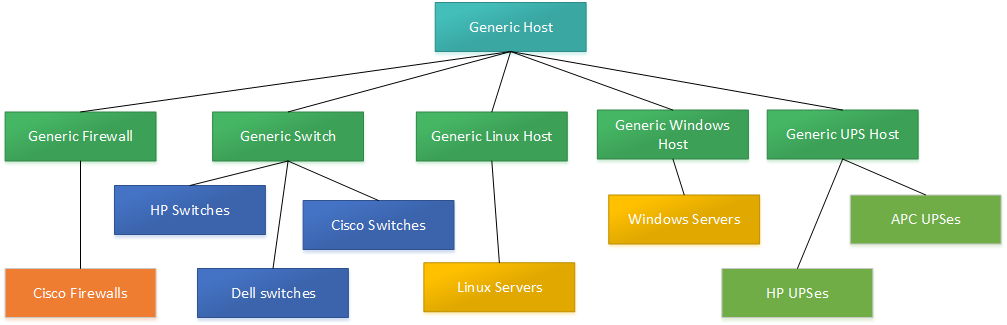
\includegraphics[scale=0.5]{img/host}
	    \caption{Oversikt over host generic plassering}
	    \label{hostfigur}
	\end{figure}

	I Figur \ref{hostgroupfigur} ser vi hvilke hostgroups de forskjellige hostene skal være medlem av.

\begin{figure}[H]
    \centering
    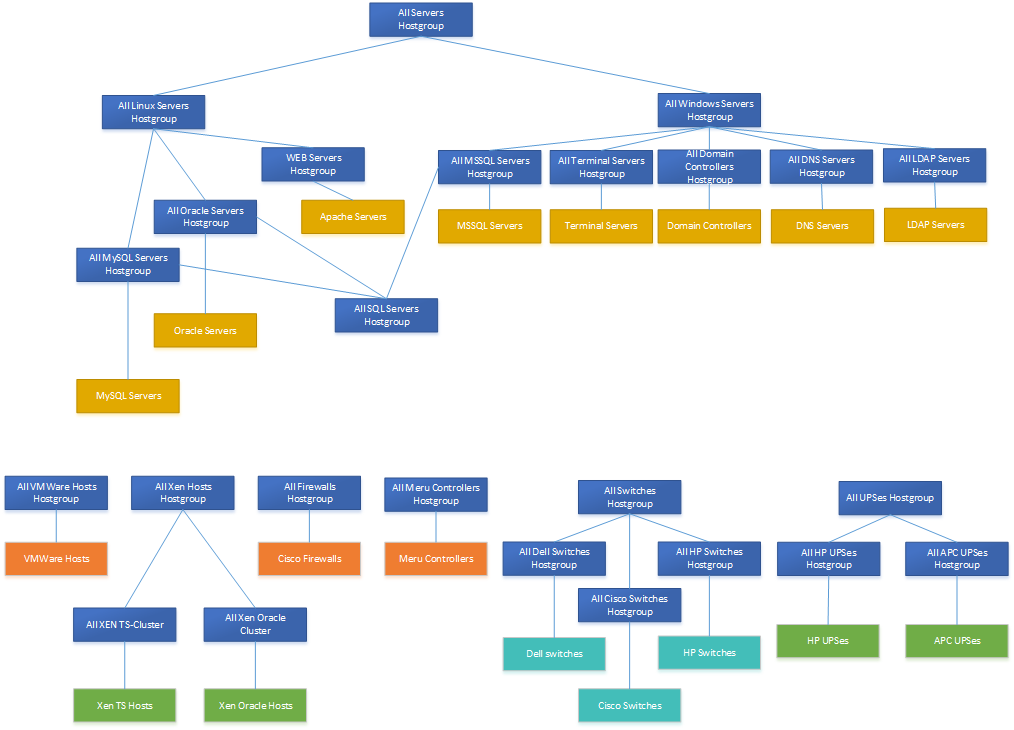
\includegraphics[scale=0.5]{img/hostgroups}
    \caption{Oversikt over host-objekter og hostgroup-plassering}
    \label{hostgroupfigur}
\end{figure}

\section{Legge til mange host-objekter}
I utrullingsfaser vil det være naturlig å legge til mange host-objekter på en gang. Ved å bruke Bash-scriptet ``gen.bash'', spares tid samtidig som scriptet sørger for at host-objektene er syntaktisk korrekte.

Scriptet genererer host-objekter med atributtene  ``hostname'', ``address'', ``hostgroup'' og ``generic''. Host-objekter uten hostgroup eller generic supplert, vil få standardverdier definert, mens hostname og address er obligatorisk, og det gis en feilmelding om disse er utelatt.

Eksempelet under viser hvordan scriptet kjøres. Linjenummer skrives ut dersom obligatorisk informasjon mangler:
\begin{lstlisting}[style=example]
monkey@hig1:~/script$ vim servers.csv
monkey@hig1:~/script$ ./gen.bash servers.csv

		Generating hosts from servers.csv into working directory

		Hostname and Address are mandatory.
		Missing for host on line nr: 4
		Missing for host on line nr: 6
		Missing for host on line nr: 7
		Missing for host on line nr: 8

		Done
		Successfully created 4 hosts
		4 hosts where not created because of errors.
	monkey@hig1:~/script$ ls
	gen.bash  servers.csv  test1.cfg  test2.cfg  test3.cfg  test4.cfg
	monkey@hig1:~/script$
	\end{lstlisting}

Koden under viser hvordan servers.csv er bygget opp. Den inneholder også feil for å vise hva som skjer dersom informasjonen ikke er korrekt:
\begin{lstlisting}
10.0.0.1,test1,windows;,generic1
10.0.0.1,test2,,jekrjekr
10.0.0.1,test3
,,,
10.0.0.1,test4
1,
,
,
\end{lstlisting}

	Kildekoden til scriptet ligger i Vedlegg \ref{gen.bash}.

\section{Forventet nedtid}
Tilfeller kan forekomme hvor en server må tas ut av drift på grunn av vedlikehold. I Icinga er det ikke nødvendig å fjerne denne fra konfigurasjonen, for å unngå at varslingsmelding blir sendt ut. I både Icinga Web og Icinga Classic har man mulighet til å bruke en funksjon som kalles ``Schedule Downtime''. Her blir nedetidens start og slutt definert.

	I den nedetidsperioden vil Icinga nekte varslingsmelding i å bli sendt ut. Når nedetidsperioden er ferdig, eller denne blir utført før avtalt tid, vil kontaktene som skal bli varslet få en melding om at nedetid er over, og Icinga vil ikke lengre holde igjen varlser.

\section{Stoppe varsling}
Når problemet som fører til et varsel for enten et host- eller service-objekt er kjent, kan en legge dette varselet i kategorien ``Acknowledged Hosts'' eller
``Acknowledged Services'' ved å benytte en kommando for gitt host- eller service-objekt i webgrensesnittet.

I Figur \ref{ackbutton} vises knappen for å sette et host- eller service-objekt acknowlegded.

	\begin{figure}[H]
	    \centering
	    
\includegraphics{img/ack_button}
	    \caption{Knapp for å settet et varsel som acknowledged}
	    \label{ackbutton}
	\end{figure}

Visning av antallet med enten WARNING eller CRITICAL vil gråtonet om bare et host- eller service-objekt er acknowledged. Tallet vil også flyttes til den midterse kolonnen som vist i Figur \ref{ackcombined} .

	\begin{figure}[H]
	    \centering
	    
\includegraphics{img/ack_combined}
	    \caption{Visning av ett acknowledged problem i webgrensesnittet}
	    \label{ackcombined}
	\end{figure}

I statusvinduet vil host- eller service-objektet legges i en egen kategori ``Known <objekttype> problems'', og ha en gråtonet farge, som vist i Figur \ref{ackstatusvindu}.

	\begin{figure}[H]
	    \centering
	    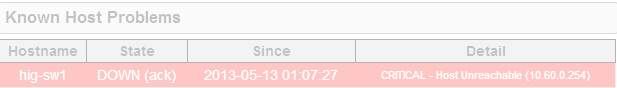
\includegraphics{img/ack_statusvindu}
	    \caption{Separering av acknowledged varsel i statusvinduet}
	    \label{ackstatusvindu}
	\end{figure}


\section{Autentisering mot Active Directory}\label{sec:ldapauth}
LDAP-autentisering brukes for å styre hvem som skal ha tilgang til webgrensesnittene, ved hjelp av grupper og brukere i Active Directory. Dette er støttet direkte i Icinga Web, men må konfigureres på andre måter for Icinga Classic. Det kan opprettes en sikkerhetsgruppe i AD som inkluderer medlemmene som skal få tilgang. Alle som er med i denne gruppen vil få tilgang til Icinga Web, der det også kan defineres hvilken informasjon hver bruker skal se. 

Selve LDAP-binden gjøres via PHP-modulen ``php-ldap''. Når en bruker logger inn sjekkes først AD, dersom brukeren ikke finnes der, vil Icinga-web prøve sin egen database med brukere. Hvis brukeren finnes her og passordet er riktig vil brukeren bli logget inn. Når brukeren har logget inn for første gang via AD, vil brukeren bli lagret i Icinga Web-databasen. Om brukeren endrer passord i Icinga Web vil uansett AD først bli spurt før Icinga Web spør om passordet er riktig i sin egen database

Icinga Classic autentiserer mot AD gjennom modulene ldap og authnz\_ldap til Apache2.

/etc/apache2/conf.d/:
\begin{lstlisting}[style=example]
    AuthName "Authentication"
    AuthType Basic
    AuthBasicProvider ldap
    AuthLDAPURL"ldap://10.60.0.22:3268/dc=monkey,dc=local?samAccountName?sub?(objectClass=person)"
    AuthLDAPBindDN "<user>"
    AuthLDAPBindPassword "<password>"
    require ldap-group CN=icinga-login, OU=icinga, DC=monkey, DC=local
\end{lstlisting}

/usr/share/icinga-web/app/modules/AppKit/config/auth.xml:
\begin{lstlisting}
    <ae:parameter name="ldap_allow_anonymous">false</ae:parameter>
        <ae:parameter name="ldap_dsn">ldap://10.60.0.22</ae:parameter>
        <ae:parameter name="ldap_start_tls">false</ae:parameter>
        <ae:parameter name="ldap_basedn">DC=monkey,DC=local</ae:parameter>
        <ae:parameter name="ldap_binddn">icingawebauth@monkey.local</ae:parameter>
        <ae:parameter name="ldap_bindpw"><![CDATA[Password]]></ae:parameter>
        <ae:parameter name="ldap_userattr">sAMAccountName</ae:parameter>
        <ae:parameter name="ldap_filter_user"><![CDATA[(&(sAMAccountName=__USERNAME__)(memberOf=CN=icinga-login,OU=icinga,DC=monkey,DC=local))]]></ae:parameter>
    </ae:parameter>
\end{lstlisting}

	\section{Kontakter og kontaktgrupper}
For å opprette en ny kontakt i Icinga meldes brukeren inn i gruppen icinga\_kontakter (hvordan dette fungerer forklart i \ref{sec:sync}). Den vil trenge å ha e-postadresse og telefonnummer satt.

Kontaktgrupper hentes fra OU-en icinga\_grupper der alle grupper hentes ut og opprettes i Icinga. For at en gruppe skal varsles må dette legges til på et service-objekt. For å slippe å sette opp kontakter for hver service kan en sende med argumentet ``gen\_service'', for å generere en template som kan benyttes på tjenester som sorterer under hver av kontaktgruppene som blir opprettet.

Eksempel på generisk service som blir opprettet:
\begin{lstlisting}[style=example]
define service {
    name 				    network_services
    register 		   		0
    use 			   		generic-service     
    notification_interval   30
    notification_period     24x7
    notification_options    w,c,r
    contact_groups          network_contact_group
}
\end{lstlisting}

Denne brukes på en Cisco firewall: 
\begin{lstlisting}[style=example]
define service {
    service_description Cisco Firewall CPU Load
    use 				network_services
    name 				cisco-firewall-cpu-load
    hostgroup_name 		all_firewalls
    check_command 		check_network_component!cpu-load
}
\end{lstlisting}

	Tabell med sjekker og tilhørende parametere:
	\begin{table}
	\begin{center}
		\begin{tabular}{| p{3cm} | l | l | l | l |}
	 \hline
		\textbf{Plugin} & \textbf{Utstyr} & \textbf{Service navn} & \textbf{Warning} & \textbf{Critical}
		\\ \hline
		\multirow{10}{*}{check\_snmp}   & APC UPS 		& UPS Capacity			& 90:	& 80: \\ \cline{2-5}
		& APC UPS			& Internal Temp			& 30	& 32 \\ \cline{2-5}
		& APC UPS			& Load				& 50	& 60 \\ \cline{2-5}
		& APC UPS			& Voltage In			& 225:239 & 220:245 \\ \cline{2-5}
		& APC UPS			& Voltage Out			& 225:239 & 220:245 \\ \cline{2-5}
		& HP UPS			& Battery Time Remaining 	& 3000: & 2700: \\ \cline{2-5}
		& HP UPS			& Battery capacity		& 90: 	& 80: \\ \cline{2-5}
		& HP UPS			& Battery current		& 	& \\ \cline{2-5}
		& HP UPS			& Voltage In			& 225:239 & 220:245 \\ \cline{2-5} 
		& HP UPS			& Voltage Out			& 225:239 & 220:245 \\ \hline
		check\_dns  & Windows Server	& Check DNS			& 0.1	& 0.2 \\ \hline
		check\_ldap & Windows Server    & Check LDAP			& 0.05	& 0.1 \\ \hline 
		\multirow{2}{*}{check\_disk}    & Windows Server		& All Disks			& 94\%	& 96\% \\ \cline{2-5}
						& Windows Server		& Disk Space			& 90\%	& 95\% \\ \hline
		check\_cpu		        & Windows Server		& CPU Load			& 90	& 95  \\ \hline
		check\_mem		        & Windows Server		& Memory Usage			& 94\%	& 98\% \\ \hline
		\multirow{2}{*}{check\_counter} & Windows Server 		& RDP-Sessions: Active		& 20	& 25 \\ \cline{2-5}
						& Windows Server		& RDP-Sessions: Inactive	& 15	& 20 \\ \hline
		\multirow{4}{*}{check\_nwc} 	& HP Procurve                   & Environment Status            & N/A   & N/A \\ \cline{2-5}
						& Cisco ASA / PIX		& CPU Load			& 93	& 96 \\ \cline{2-5}
						& Cisco ASA / PIX 		& Memory Usage			& 93    & 96 \\ \cline{2-5}
						& Cisco ASA / PIX		& Hardware Health		& N/A	& N/A \\ \hline
		check\_cisco\_ failover		& Cisco ASA / PIX		& Failover Status		& N/A	& N/A \\ \hline
		check\_asa\_vpn			& Cisco ASA / PIX		& VPN Sessions		 & 80 (\% av lisens) & 90 (\% av lisens) \\ \hline
		check\_dell\_ bladechassis	& Dell Blade Chassis		& Dell Blade Server Health	& N/A	& N/A \\ \hline
		\multirow{5}{2cm}{check\_snmp\_ powerconnect} & Dell Powerconnect	& Assets			& N/A	& N/A \\ \cline{2-5}
							   & Dell Powerconnect	& Uptime			& N/A	& N/A \\ \cline{2-5}
							   & Dell Powerconnect	& Fans				& N/A	& N/A \\ \cline{2-5}
							   & Dell Powerconnect	& Power supply			& N/A	& N/A \\ \cline{2-5}
							   & Dell Powerconnect	& Temperature			& 34	& 36 \\ \hline
		\multirow{4}{2cm}{check\_mysql\_ health}      & MySQL			& Cache Hit			& 60: 	& 50: \\ \cline{2-5}
							   & MySQL			& Health			& 0.1	& 0.2 \\ \cline{2-5}
							   & MySQL			& Slow Queries			& 0.1	& 1 \\ \cline{2-5}
							   & MySQL			& User Connections		& 50	& 80 \\ \hline
		\multirow{4}{2cm}{check\_mssql\_ health}	   & MSSQL			& Cache Hit			& 90:	& 80: \\ \cline{2-5}
							   & MSSQL			& Health			& 0.05	& 0.15 \\ \cline{2-5}
							   & MSSQL			& Lazy Writes			& 20	& 0 \\ \cline{2-5}
							   & MSSQL			& User Connections		& 2000	& 2200 \\ \hline
		\multirow{4}{2cm}{check\_oracle\_ health}	   & Oracle			& Cache Hit			& 93:	& 90: \\ \cline{2-5}
							   & Oracle			& Connected Users		& 50	& 80 \\ \cline{2-5}
							   & Oracle			& Connection Time		& 0.1	& 0.2 \\ \cline{2-5}
							   & Oracle			& Free Tablespace		& 5:	& 2: \\ \hline
\end{tabular}
\label{plugins_parametere}
\end{center}
\end{table}

\section{Backup-rutiner}
I Tabell \ref{backup}, vises viktige filer og mapper for overvåkningsløsningen. Disse bør integreres i en backup av Icinga-serveren.
\begin{table} \label{backup}
\begin{center}
\begin{tabular}{| p{8cm} | p{8cm} |}
 \hline
        \textbf{Filbane} & \textbf{Inneholder}
	\\ \hline
	/etc/icinga/ & Alle konfigurasjonsfiler for Icinga \\ \hline
	/usr/lib/nagios/plugins/ & Alle plugin-er \\ \hline
	/etc/nagios-plugins/config & Konfigurasjon for default plugins \\ \hline
	/root/Scripts & Lokale script. \\ \hline
	/etc/snmp & Konfigurasjon for snmptt \\ \hline
	/etc/default/snmp & Konfigurasjon for at snmpd starter snmptrapd \\ \hline
	/etc/sysconfig/icinga & Konfigurasjon for environment variabler \\ \hline
	/usr/lib/oracle/11.2/client64/network/
	admin/tnsnames.ora & Konfigurasjon for oracle-instanser \\ \hline
	/etc/init.d/carbon-cache & Init script for grafprosessering gjennom graphite \\ \hline
	/etc/init.d/metricinga & Init script for prosessering av perfdata fra Icinga \\ \hline
	/opt/graphite/ & Konfigurasjon og data for genering av grafer  \\ \hline
\end{tabular}
\end{center}
\end{table}
I tilegg bruker Icinga Classic og Icinga Web hver sine databaser, kalt ``icinga'' og ''icinga\_web''. Graphite bruker også en database, som heter ``graphite''.
